\documentclass[english,floatsintext,man]{apa6}

\usepackage{amssymb,amsmath}
\usepackage{ifxetex,ifluatex}
\usepackage{fixltx2e} % provides \textsubscript
\ifnum 0\ifxetex 1\fi\ifluatex 1\fi=0 % if pdftex
  \usepackage[T1]{fontenc}
  \usepackage[utf8]{inputenc}
\else % if luatex or xelatex
  \ifxetex
    \usepackage{mathspec}
    \usepackage{xltxtra,xunicode}
  \else
    \usepackage{fontspec}
  \fi
  \defaultfontfeatures{Mapping=tex-text,Scale=MatchLowercase}
  \newcommand{\euro}{€}
\fi
% use upquote if available, for straight quotes in verbatim environments
\IfFileExists{upquote.sty}{\usepackage{upquote}}{}
% use microtype if available
\IfFileExists{microtype.sty}{\usepackage{microtype}}{}

% Table formatting
\usepackage{longtable, booktabs}
\usepackage{lscape}
% \usepackage[counterclockwise]{rotating}   % Landscape page setup for large tables
\usepackage{multirow}		% Table styling
\usepackage{tabularx}		% Control Column width
\usepackage[flushleft]{threeparttable}	% Allows for three part tables with a specified notes section
\usepackage{threeparttablex}            % Lets threeparttable work with longtable

% Create new environments so endfloat can handle them
% \newenvironment{ltable}
%   {\begin{landscape}\begin{center}\begin{threeparttable}}
%   {\end{threeparttable}\end{center}\end{landscape}}

\newenvironment{lltable}
  {\begin{landscape}\begin{center}\begin{ThreePartTable}}
  {\end{ThreePartTable}\end{center}\end{landscape}}




% The following enables adjusting longtable caption width to table width
% Solution found at http://golatex.de/longtable-mit-caption-so-breit-wie-die-tabelle-t15767.html
\makeatletter
\newcommand\LastLTentrywidth{1em}
\newlength\longtablewidth
\setlength{\longtablewidth}{1in}
\newcommand\getlongtablewidth{%
 \begingroup
  \ifcsname LT@\roman{LT@tables}\endcsname
  \global\longtablewidth=0pt
  \renewcommand\LT@entry[2]{\global\advance\longtablewidth by ##2\relax\gdef\LastLTentrywidth{##2}}%
  \@nameuse{LT@\roman{LT@tables}}%
  \fi
\endgroup}


  \usepackage{graphicx}
  \makeatletter
  \def\maxwidth{\ifdim\Gin@nat@width>\linewidth\linewidth\else\Gin@nat@width\fi}
  \def\maxheight{\ifdim\Gin@nat@height>\textheight\textheight\else\Gin@nat@height\fi}
  \makeatother
  % Scale images if necessary, so that they will not overflow the page
  % margins by default, and it is still possible to overwrite the defaults
  % using explicit options in \includegraphics[width, height, ...]{}
  \setkeys{Gin}{width=\maxwidth,height=\maxheight,keepaspectratio}
\ifxetex
  \usepackage[setpagesize=false, % page size defined by xetex
              unicode=false, % unicode breaks when used with xetex
              xetex]{hyperref}
\else
  \usepackage[unicode=true]{hyperref}
\fi
\hypersetup{breaklinks=true,
            pdfauthor={},
            pdftitle={Word Learning as Network Growth: A Cross-linguistic Analysis},
            colorlinks=true,
            citecolor=blue,
            urlcolor=blue,
            linkcolor=black,
            pdfborder={0 0 0}}
\urlstyle{same}  % don't use monospace font for urls

\setlength{\parindent}{0pt}
%\setlength{\parskip}{0pt plus 0pt minus 0pt}

\setlength{\emergencystretch}{3em}  % prevent overfull lines

\ifxetex
  \usepackage{polyglossia}
  \setmainlanguage{}
\else
  \usepackage[english]{babel}
\fi

% Manuscript styling
\captionsetup{font=singlespacing,justification=justified}
\usepackage{csquotes}
\usepackage{upgreek}

 % Line numbering
  \usepackage{lineno}
  \linenumbers


\usepackage{tikz} % Variable definition to generate author note

% fix for \tightlist problem in pandoc 1.14
\providecommand{\tightlist}{%
  \setlength{\itemsep}{0pt}\setlength{\parskip}{0pt}}

% Essential manuscript parts
  \title{Word Learning as Network Growth: A Cross-linguistic Analysis}

  \shorttitle{Word Learning as Network Growth}


  \author{Abdellah Fourtassi\textsuperscript{1}, Yuan Bian\textsuperscript{2}, \& Michael C. Frank\textsuperscript{1}}

  % \def\affdep{{"", "", ""}}%
  % \def\affcity{{"", "", ""}}%

  \affiliation{
    \vspace{0.5cm}
          \textsuperscript{1} Department of Psychology, Stanford University\\
          \textsuperscript{2} Department of Psychology, University of Illinois  }

  \authornote{
    Abdellah Fourtassi
    
    Department of Psychology
    
    Stanford University
    
    50 Serra Mall
    
    Jordan Hall, Building 420
    
    Stanford, CA 94301
    
    Correspondence concerning this article should be addressed to Abdellah
    Fourtassi, Postal address. E-mail:
    \href{mailto:afourtas@stanford.edu}{\nolinkurl{afourtas@stanford.edu}}
  }


  \abstract{Children tend to produce words earlier when they are connected to a
variety of other words along both the phonological and semantic
dimensions. Though this connectivity effect has been extensively
documented, little is known about the underlying developmental
mechanism. One view suggests that learning is primarily driven by a
network growth model where highly connected words in the child's early
lexicon attract similar words. Another view suggests that learning is
driven by highly connected words in the external learning environment
instead of highly connected words in the early internal lexicon. The
present study tests both scenarios systematically in both the
phonological and semantic domains, and across 8 languages. We show that
external connectivity in the learning environment drives growth in both
the semantic and the phonological networks, and that this pattern is
consistent cross-linguistically. The findings suggest a word learning
mechanism where children harness their statistical learning abilities to
(indirectly) detect and learn highly connected words in the learning
environment.}
  \keywords{Language understanding; audio-visual processing; word learning; speech
perception; computational modeling. \\

    
  }




  \usepackage[sortcites=false,sorting=none]{biblatex}

\usepackage{amsthm}
\newtheorem{theorem}{Theorem}
\newtheorem{lemma}{Lemma}
\theoremstyle{definition}
\newtheorem{definition}{Definition}
\newtheorem{corollary}{Corollary}
\newtheorem{proposition}{Proposition}
\theoremstyle{definition}
\newtheorem{example}{Example}
\theoremstyle{definition}
\newtheorem{exercise}{Exercise}
\theoremstyle{remark}
\newtheorem*{remark}{Remark}
\newtheorem*{solution}{Solution}
\begin{document}

\maketitle

\setcounter{secnumdepth}{0}



\section{Introduction}\label{introduction}

What factors shape vocabulary learning over the course of early
childhood? To investigate this question, scientists have adopted
multiple research strategies, from conducting controlled laboratory
experiments (e.g. Markman, 1990) to analyzing dense corpora capturing
language learning in context (e.g., B. C. Roy, Frank, DeCamp, Miller, \&
Roy, 2015). One strategy consists in documenting the timeline of words'
acquisition, and studying the properties that make words easy or hard to
learn. For example, within a lexical category, words that are more
frequent in child-directed speech are acquired earlier (J. C. Goodman,
Dale, \& Li, 2008). Other factors include word length, the mean length
of utterances in which the word occurs, and concreteness (see Braginsky,
Yurovsky, Marchman, \& Frank, 2016).

Besides these word-level properties, the lexical structure (that is, how
words relate to each other) also influences the age of acquisition of
words. The lexical structure is best characterized in terms of a network
where each node represents a word in the vocabulary, and each link
between two nodes represents a relationship between the corresponding
pair of words. Previous studies have investigated early vocabulary
structure by constructing networks using a variety of word-word
relations including shared semantic features, target-cue relationships
in free association norms, co-occurrence in child directed speech, and
phonological similarity. These studies have found that children tend to
produce words that have higher neighborhood density (i.e., high
connectivity in the network) earlier, both at the phonological and the
semantic level (Engelthaler \& Hills, 2017; Hills, Maouene, Riordan, \&
Smith, 2010; Hills, Maouene, Maouene, Sheya, \& Smith, 2009; Stella,
Beckage, \& Brede, 2017; Storkel, 2009).

While most studies have focused on the static properties of the lexical
network, a few have investigated the underlying developmental process.
In particular, Steyvers and Tenenbaum (2005) suggested that the observed
effects of connectivity are the consequence of how the lexical network
gets constructed in the child's mind. According to this explanation,
known as Preferential Attachment (PAT), highly connected words in the
child's lexicon tend to \enquote{attract} more words over time, in a
rich-get-richer scenario (Barabasi \& Albert, 1999). In other words,
what predicts word learning is the \emph{internal} connectivity in the
child's early lexicon. In contrast, Hills et al. (2009) suggested that
what biases the learning is not the connectivity in the child's internal
lexicon but, rather, \emph{external} connectivity in the learning
environment. They called this alternative explanation Preferential
Acquisition (PAC). Figure~\ref{fig:growth} shows an illustration of both
growth scenarios with the same simplified network. These two proposals
represent two divergent ideas about the role of lexical networks in
acquisition. On the PAT proposal, network structure is a causal factor
in early word learning; in contrast, on the PAC approach, network
structure is not internally represented and, therefore, might be an
epiphenomenon of the statistics of the linguistic input.

\begin{figure}

{\centering 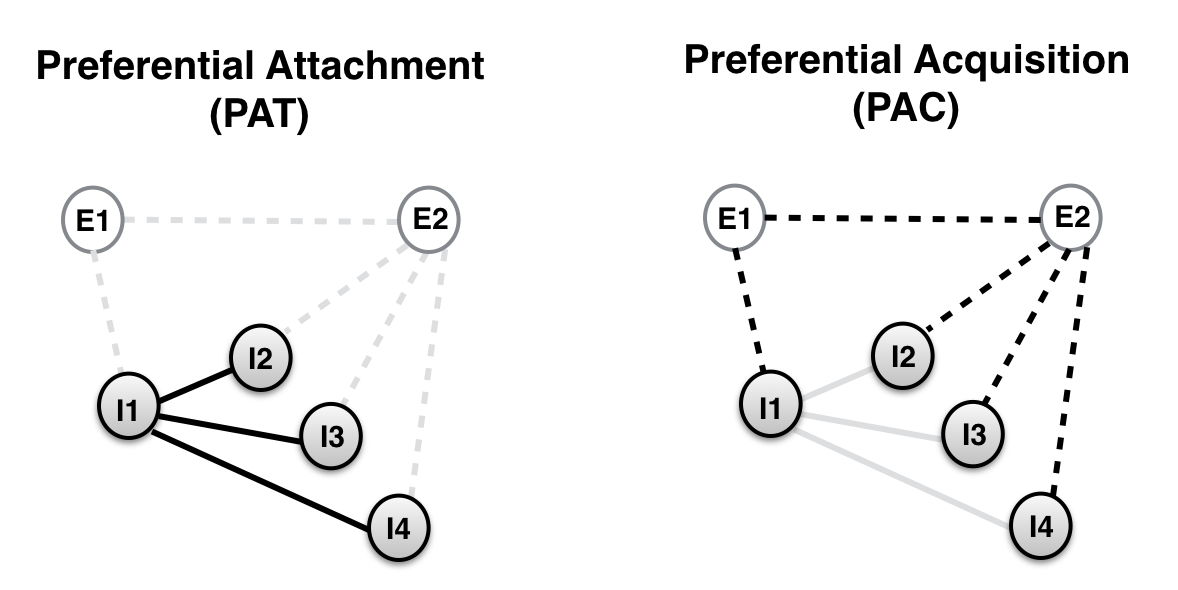
\includegraphics[width=400px]{figs/growth2} 

}

\caption{Illustration of the growth scenarios. Filled circles (I1-I4) represent known words (internal), and empty circles (E1 and E2) represent words that have not been learned yet (external). Black lines represent links that are relevant in each growth scenario, and gray lines represent links that are irrelevant. For PAT, the utility of a candidate, external node is the average degree (i.e., number of links) of the internal nodes that it would attach to. Thus, according to PAT, the node E1 is more likely to enter the lexicon first. For PAC, the utility of a candidate node is its degree in the entire network. According to PAC, the node E2 is more likely to enter the lexicon first.}\label{fig:growth}
\end{figure}

Studies that investigate lexical network growth have focused on semantic
networks using English data (Hills et al., 2010, 2009; Steyvers \&
Tenenbaum, 2005). The novelty of the current study is threefold: First,
it investigates whether phonological networks, like semantic networks,
grow by PAC, or if they rather grow by PAT. Second, it provides a
systematic comparison of both network growth scenarios in the
phonological and the semantic domains and assesses their relative
contribution to the learning process. Third, it tests the generality of
the findings across eight languages.

\section{Networks}\label{networks}

\subsection{Data}\label{data}

We used data from Wordbank (Frank, Braginsky, Yurovsky, \& Marchman,
2017), an open repository aggregating cross-linguistic language
developmental data of the MacArthur-Bates Communicative Development
Inventory (CDI), a parent report vocabulary checklist. Parent report is
a reliable and valid measure of children's vocabulary that allows for
the cost-effective collection of datasets large enough to test
network-based models of acquisition (Fenson et al., 1994). We used the
\emph{Words and Sentences} version of the CDI which contains the
productive vocabulary of toddlers (age varied between 16 to 36 months).
Following previous studies (Hills et al., 2009; Storkel, 2009), we
restricted our analysis to nouns. We defined the age of acquisition of a
given word by the month at which this word was produced by at least 50\%
of children (J. C. Goodman et al., 2008), and we excluded nouns that
have not been learned (according to this criterion) by the last month
for which we have CDI data.

We obtained these nouns in eight languages: Croatian, Danish, English,
Italian, Norwegian, Russian, Spanish, and Turkish. We used the subset of
nouns that had entries in the Florida Association Norms (see below).
Since these norms are available only in English, we used the
hand-checked translation equivalents provided by Braginsky et al.
(2016), allowing us to use the English association norms across
languages. Table \ref{tab:stats} gives an overview of the data used.
Translation equivalents were originally constructed for a subset of
words appearing on the toddler CDI form, and so not all words are
currently available. Note, however, that all languages have at least
60\% of nouns translated.

\begin{table}[H]
\centering
\begin{tabular}{rlrrr}
  \hline
 & language & total & translated & normed \\ 
  \hline
1 & Croatian & 253 & 177 & 170 \\ 
  2 & Danish & 295 & 198 & 187 \\ 
  3 & English & 296 & 296 & 274 \\ 
  4 & Italian & 311 & 203 & 194 \\ 
  5 & Norwegian & 305 & 193 & 186 \\ 
  6 & Russian & 311 & 311 & 285 \\ 
  7 & Spanish & 240 & 173 & 163 \\ 
  8 & Turkish & 293 & 175 & 164 \\ 
   \hline
\end{tabular}
\caption{\label{tab:stats}Total number of nouns produced by toddlers in the CDI (left). We included in our study the subset of these nouns that had available English translations (middle). The final set consisted of nouns that had both available translations as well entries in the Free Association Norms (right).} 
\end{table}

\section{Semantic networks}\label{semantic-networks}

We constructed semantic networks following the procedure outlined in
Hills et al. (2009). We used as an index of semantic relatedness the
Florida Free Association Norms (Nelson, McEvoy, \& Schreiber, 1998).
This dataset was collected by giving adult participants a word (the
cue), and asking them to write the first word that comes to mind (the
target). For example, when given the word \enquote{ball}, they might
answer with the word \enquote{game}. A pair of nodes were connected by a
directed link from the cue to the target if there was a cue-target
relationship between these nodes in the association norms. The
connectivity of a given node was characterized by its \emph{indegree}:
the number of links for which the word was the target. To model growth
from month to month, we constructed a different network at each month,
based on the words that have been acquired by that month.

\subsection{Phonological networks}\label{phonological-networks}

We generated approximate International Phonetic Alphabet (IPA)
transcriptions from the orthographic transcription, across languages,
using the open source text-to-speech software
\textbf{\href{http://http://espeak.sourceforge.net/}{Espeak}.} We used
the Levenshtein distance (also known as edit distance) as a measure of
phonological relatedness between two nodes. The measure counts the
minimum number of operations (insertions, deletions, substitutions)
required to change one string into another.

In previous studies, two nodes were linked if they had an edit distance
of 1 (e.g., Storkel, 2009). However, in these previous studies the
network was built using an adult vocabulary. In the current study,
however, network growth models are based on the children's early
vocabulary which contains very few word pairs with an edit distance of
1. When using this threshold, the resulting networks were too sparse and
uninformative. Thus, we increased the threshold from 1 to 2, that is,
two nodes were related if their edit distance was equal to 1 or 2. The
connectivity of a given node was characterized with its \emph{degree}:
the number of links it shares with other words.

\section{Analysis}\label{analysis}

\subsection{Static properties of the global
network}\label{static-properties-of-the-global-network}

We start by analyzing word connectivity in the global (static) network.
We constructed this network using nouns learned by the oldest age for
which we have CDI data (e.g., in English this corresponds to the network
by 30 months). This global network is the end-state towards which both
PAT and PAC should converge by the last month of learning. Moreover,
following Hills et al. (2009), we used this end-state network as a proxy
for the external connectivity in the learning environment. Below we
analyze properties of this global networks that are relevant to PAC
and/or PAT.

\begin{figure}[!h]
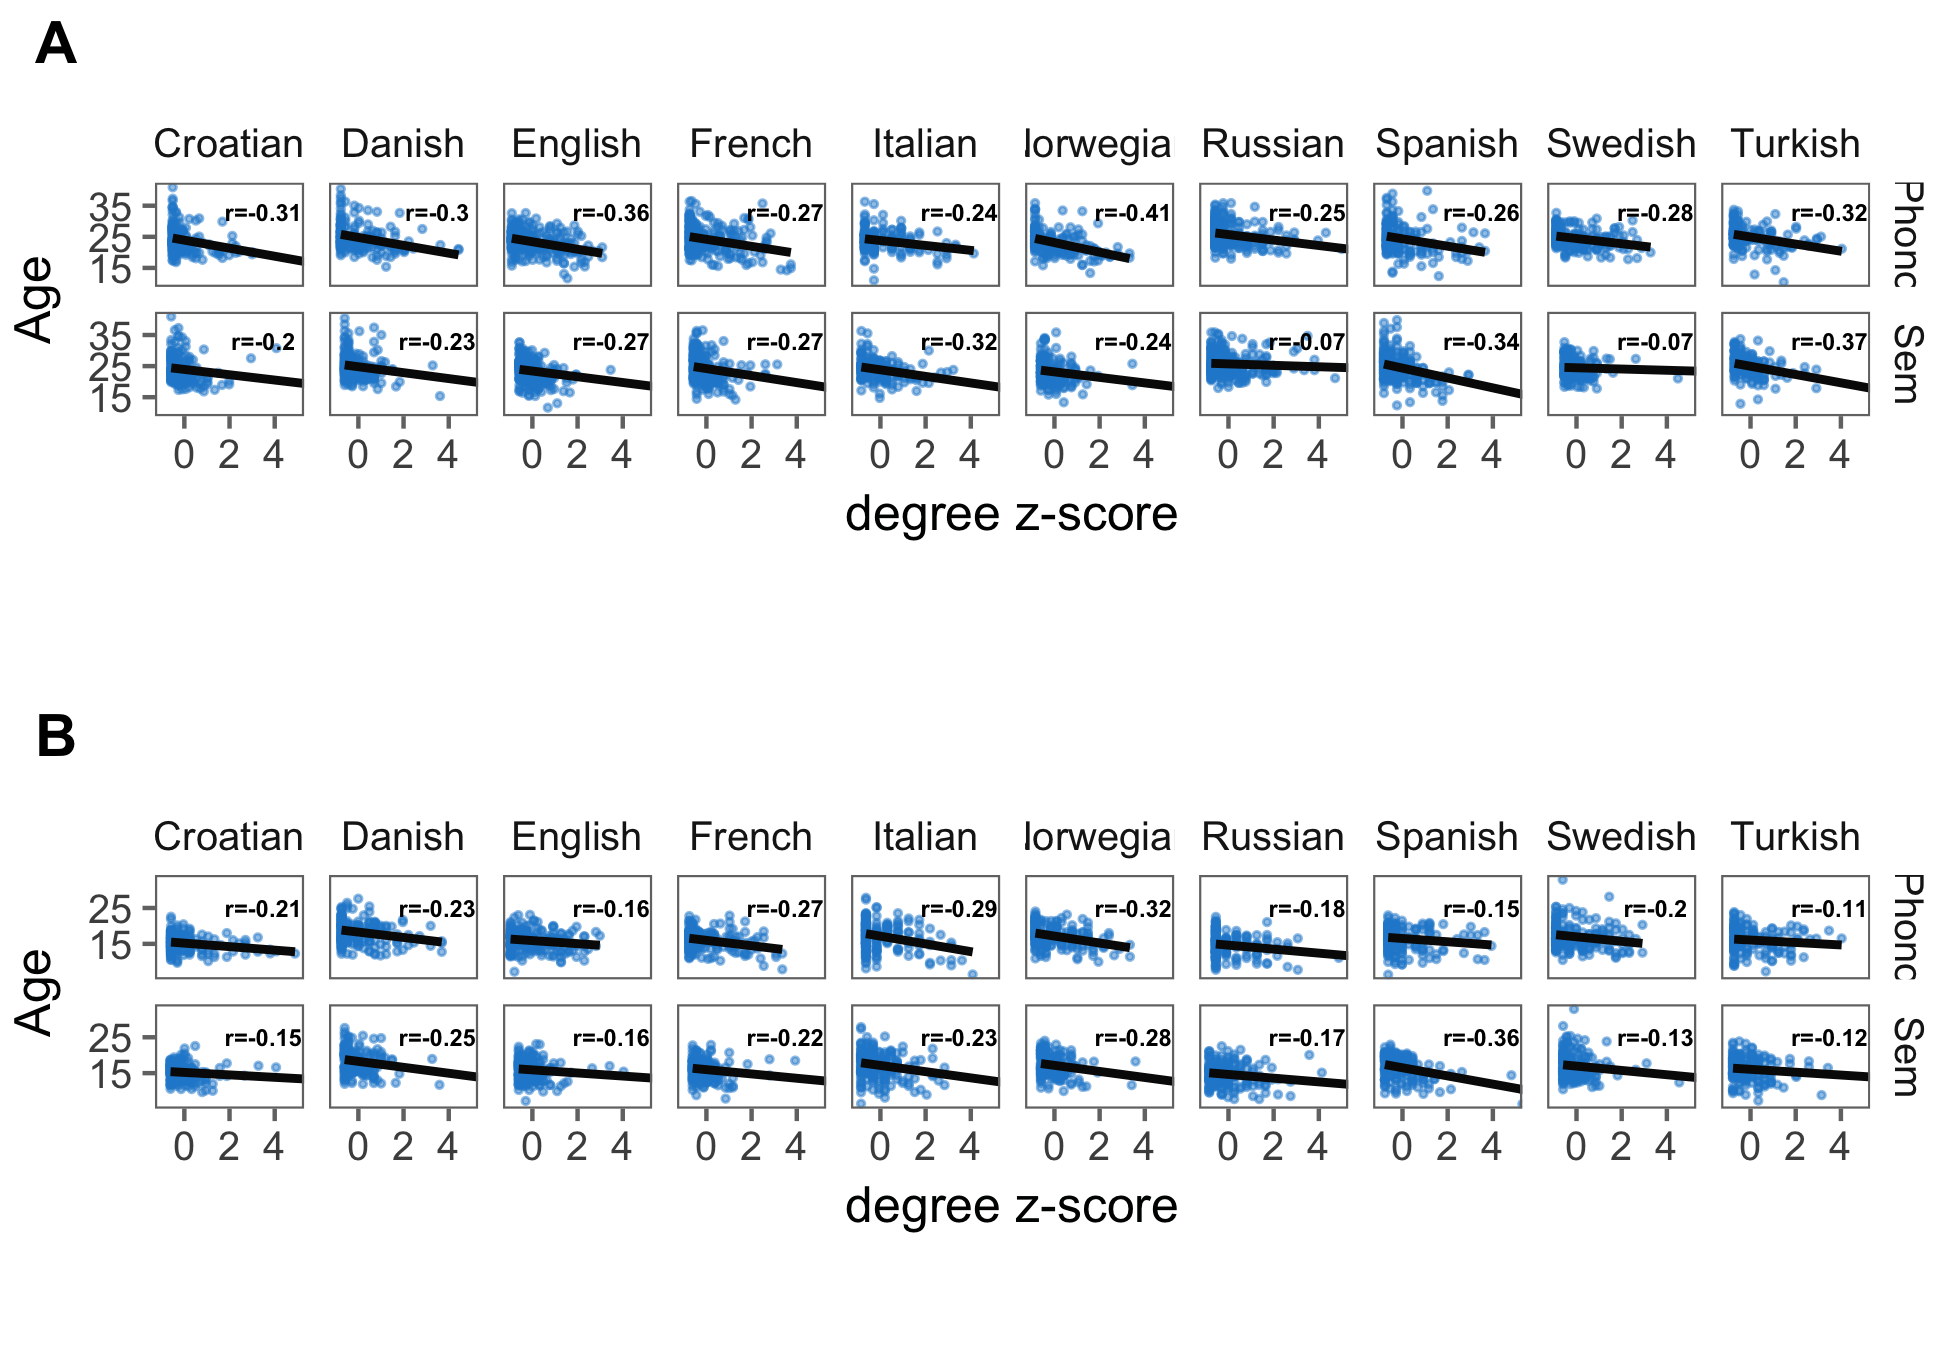
\includegraphics[width=\textwidth]{ms_files/figure-latex/corrAll-1} \caption{Age of production (A) and comprehension (B) in the global network as predicted by the degree in this network. Results are shown in each language for phonological and semantic networks. Each point is a word, with lines indicating linear model fits.}\label{fig:corrAll}
\end{figure}

\subsubsection{Connectivity predicts the age of
acquisition}\label{connectivity-predicts-the-age-of-acquisition}

Connectivity in the global network is directly related to PAC as it
represents the explicit criterion PAC uses to determine what words
should be learned first (Figure \ref{fig:growth}). Therefore, a direct
consequence of a PAC-like growth scenario is a correlation between
connectivity in the global network and the age of
acquisition.\footnote{This correlation is also compatible with PAT, although the causality is reversed. Indeed, from the perspective of this growth scenario, higher connectivity in the global network is caused by earlier learning, not the other way around. Some words end up being highly connected in the global network precisely because they happen to be acquired earlier and, therefore, have a higher chance of accumulating more links over time.}
Figure \ref{fig:corrAll} shows how the age of production (A) and
comprehension (B) for each word varies as a function of its degree (or
indegree for the semantic network). For ease of visual comparison, the
predictor (i.e., the degree) was centered and scaled across languages.
The plots show, overall, a negative correlation between the month of
acquisition and the degree, indicating that nouns with higher degrees
are generally learned earlier.

\begin{figure}[!h]
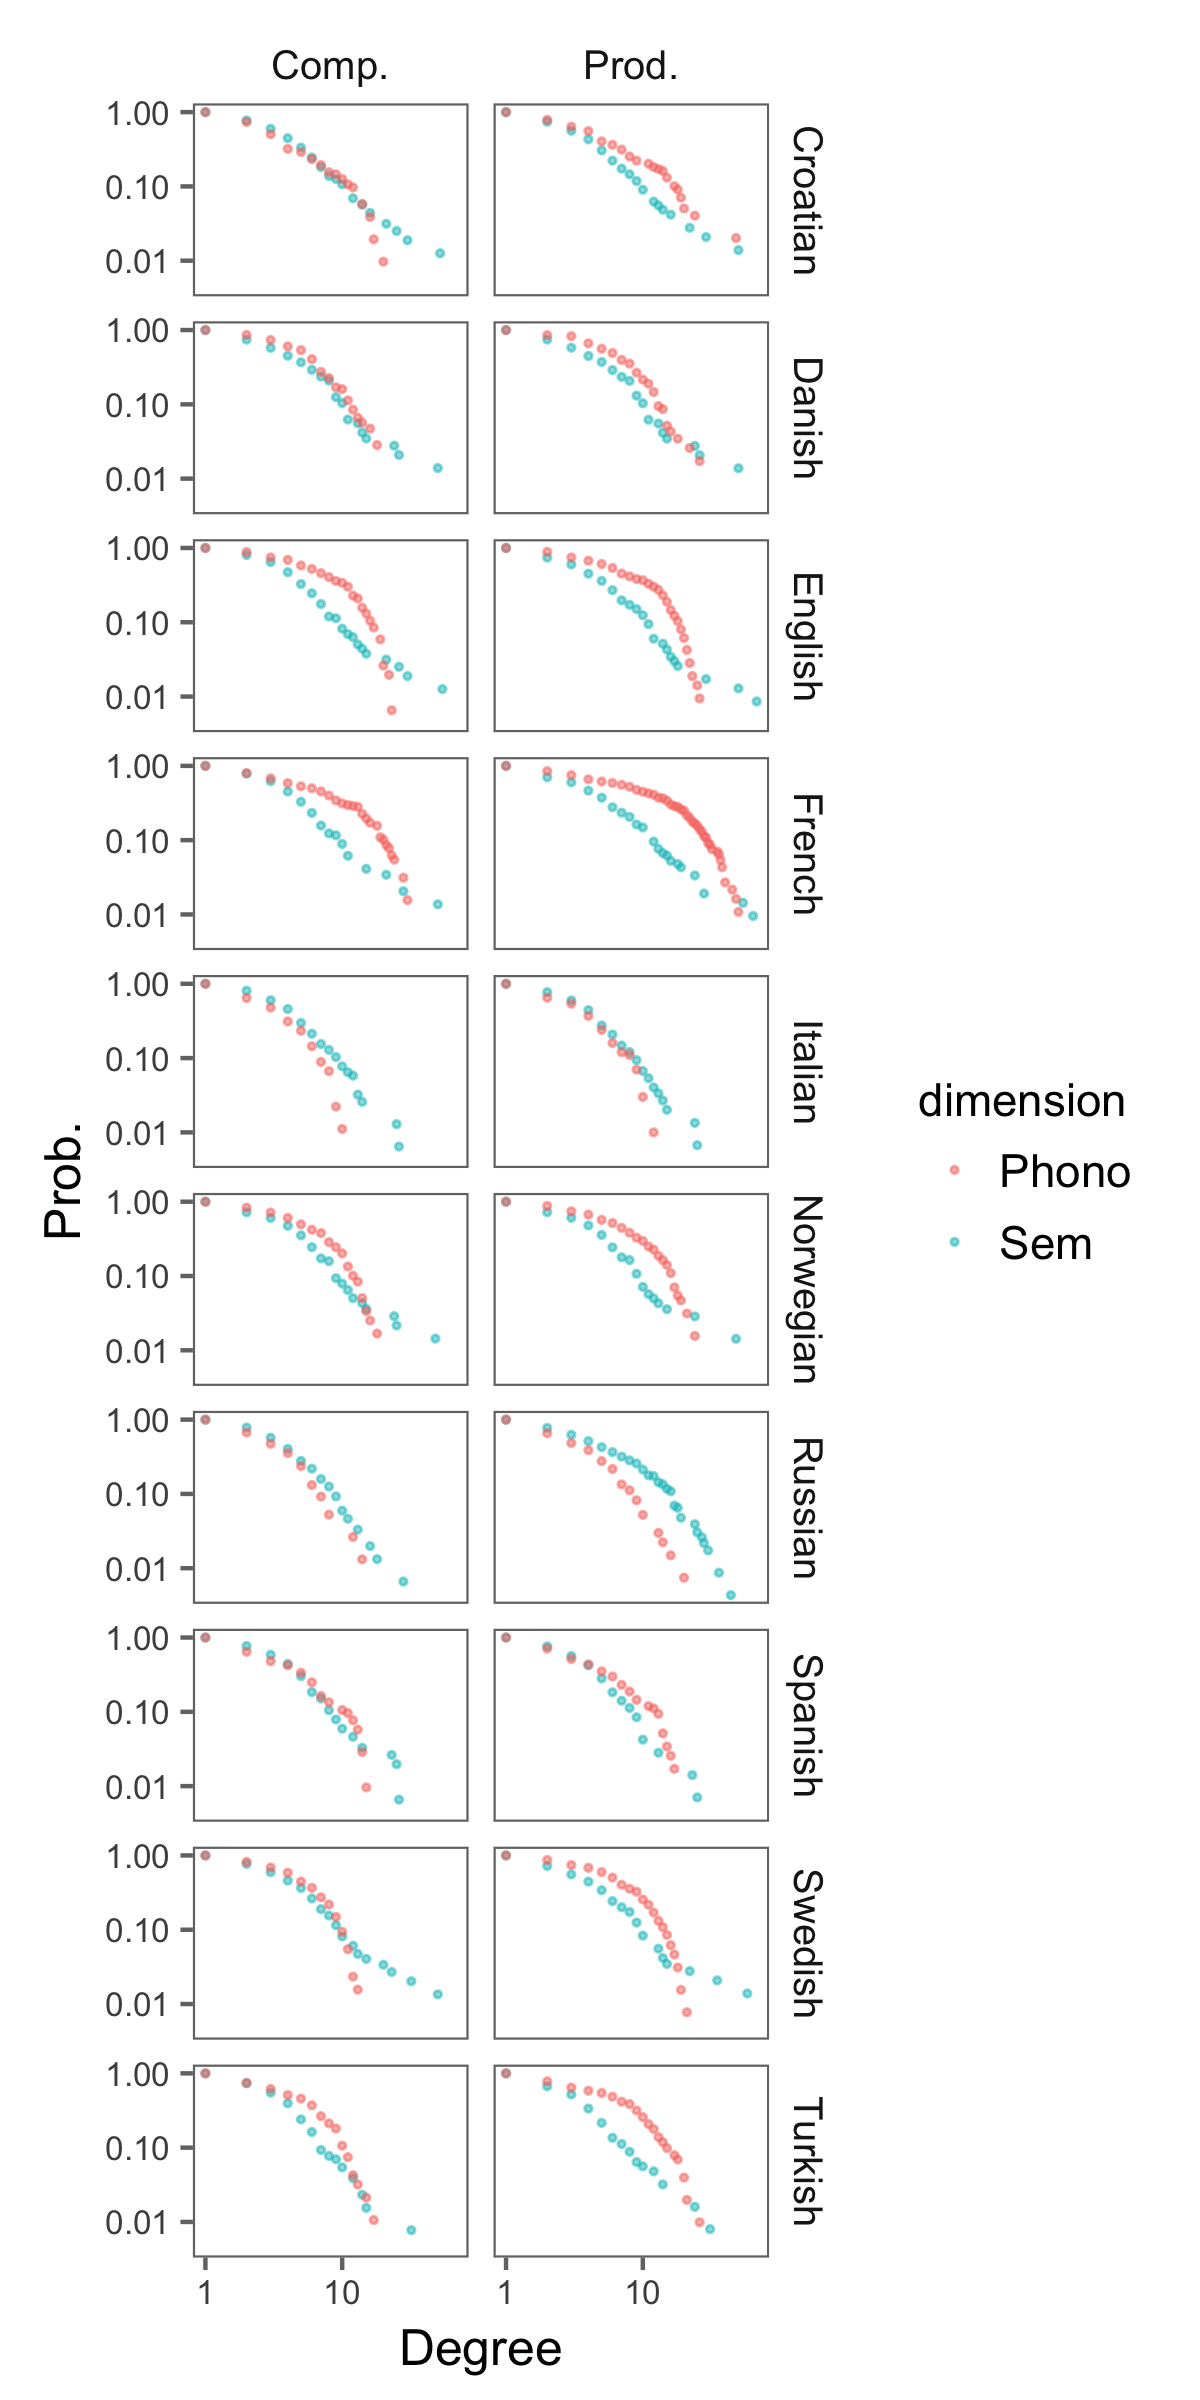
\includegraphics[width=\textwidth]{figs/plot_degree} \caption{Log-log plot of the cumulative degree distribution function for the global phonological and semantic networks across languages. The figure shows the results for both production and comprehension data. A perfect power-law distribution should appear as a straight line in this graph.}\label{fig:degreeDist}
\end{figure}

\subsubsection{Power-law degree
distribution?}\label{power-law-degree-distribution}

We also analyzed the global network's degree distribution. The shape of
this distribution is particularly relevant to PAT as this growth
scenario is known to generate networks with a power-law degree
distribution (i.e., a distribution of the form
\(p(k) \propto \frac{1}{k^{\alpha}}\), Barabasi \& Albert, 1999). If the
network displays this property, this fact would suggest a PAT-like
generative process. Conversely, if the degree distribution does not
follow a power law, this fact would weaken the case for PAT. The log-log
plots are shown in Figure \ref{fig:degreeDist}. We fit a power law to
each empirical degree distribution following the procedure outlined in
Clauset, Shalizi, and Newman (2009) and using the related R package
(poweRlaw, Gillespie, 2015). In brief, the analysis consisted in two
steps. First, we derived the optimal cut-off, \(k_{min}\), above which
the distribution is more likely to follow a power
law,\footnote{In natural phenomena, it is often the case that the power law applies only for values above a certain minimum.}
and we estimate the corresponding scaling parameter \(\alpha\). Second
we calculated the goodness-to-fit, which resulted in a \(p\)-value
quantifying the plausibility of the model. The results are shown in
Appendix 1, table XX. Overall, we could not reject the null hypothesis
of a power-law distribution: the \(p\)-value was generally above 0.1.

In sum, the static properties of the global network are \emph{a priori}
compatible with both PAT and PAC. In order to decide between these two
developmental scenarios, we need to fit explicit growth models to the
data.

\begin{figure}[!h]
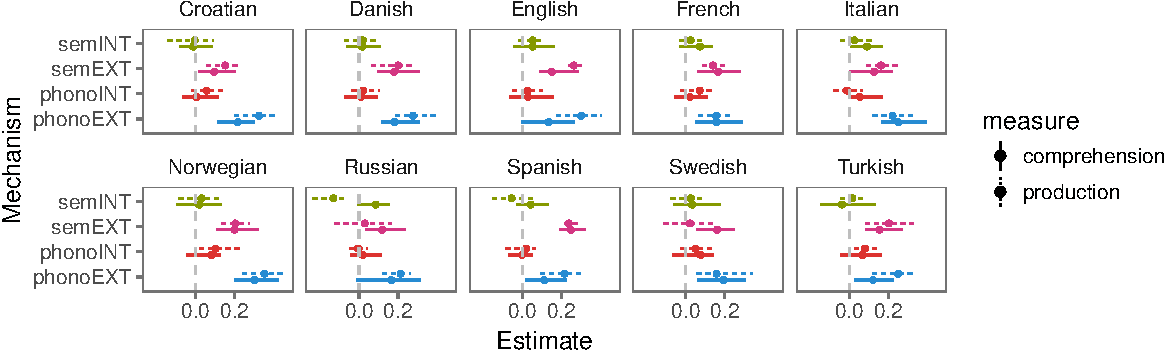
\includegraphics[width=\textwidth]{ms_files/figure-latex/growthPred-1} \caption{Evaluation of growth scenarios (EXT: externally-driven, INT: internally-driven) for both semantic and phonological networks. Each point represents the mean of the posterior distribution of the growth parameter, with ranges representing 95\% credible intervals. Positive values mean that learning proceeds according to the predictions of the growth scenario, whereas negative values mean that learning proceeds in opposition to the predictions of the growth scenario.}\label{fig:growthPred}
\end{figure}

\subsection{Network growth models}\label{network-growth-models}

\subsubsection{How does each growth scenario predict noun
development?}\label{how-does-each-growth-scenario-predict-noun-development}

To test the network growth scenarios, we fit different growth models to
the data. We calculated the probability that a word \(w_i\), with a
growth value \(d_i\) would enter the lexicon at a given month, using a
softmax function:

\begin{equation}
 p(w_i)= \frac{e^{\beta d_i}}{\sum_j e^{\beta d_j} }
\end{equation}

\noindent where \(\beta\) is a fitted parameter that captures the
magnitude of the relationship between network parameters and growth
(analogous to a regression coefficient). A positive value of \(\beta\)
means that words with higher growth values \(d_i\) are acquired first,
and a negative value means that words with lower growth values are
acquired first (see Figure \ref{fig:growth} for an illustration of how
growth values \(d_i\) are defined in each growth scenario). The
normalization includes all words that could be learned at that month.

We estimated the parameter \(\beta\) using a Bayesian approach. The
inference was performed using the probabilistic programming language
WebPPL (N. Goodman \& Stuhlmuller, 2014). We defined a uniform prior
over \(\beta\), and at each month, we computed the likelihood function
over words that could possibly enter the lexicon at that month, fit to
the words that have been learned at that month (using formula 1). Markov
Chain Monte Carlo sampling resulted in a posterior distribution over
\(\beta\), which we summarized in Figure \ref{fig:growthPred}.

For the semantic networks, the results replicate Hills et al.'s finding
in English, which is that the semantic network grows by PAC, not by PAT.
Moreover, this finding holds in seven of the eight languages we
examined.\footnote{One could imagine that the fact of using English free association norms cross-linguistically would decrease the effect of non-English semantic networks because of possible cultural differences. However, our findings do not support this assumption as the effects were generally similar in magnitude cross-linguistically.}
The PAC model also fits better than PAT for phonological networks. We
note however that PAT, though weaker, fares better for the phonological
networks (where it predicts part of the growth process in some languages
such as Croatian, English, Norwegian and Russian) than it does for the
semantic networks (where it is rather universally unpredictive).

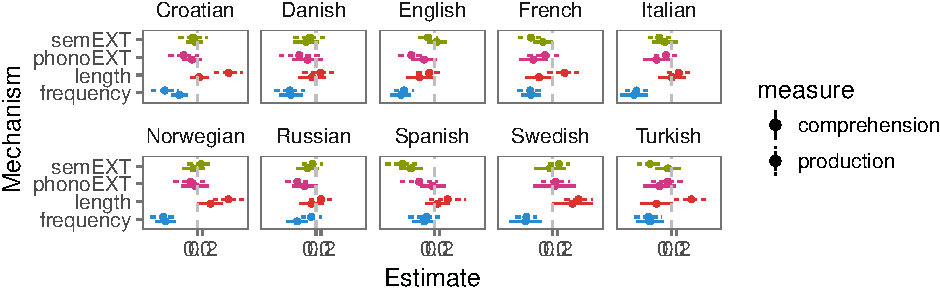
\includegraphics{ms_files/figure-latex/unnamed-chunk-6-1.pdf}

\begin{figure}[!h]
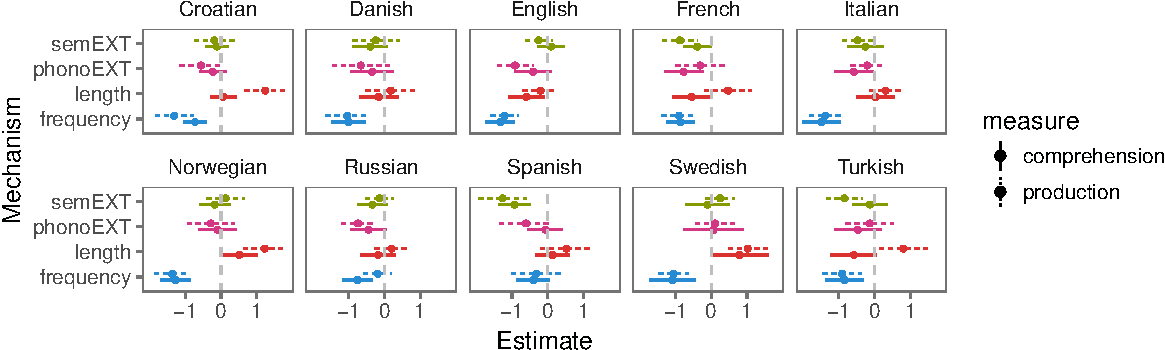
\includegraphics[width=\textwidth]{ms_files/figure-latex/staticPred-1} \caption{Estimates of the relative contribution of each predictor of AoA in the combined regression model. Results are shown for both production and comprehension data. Ranges indicate 95\% confidence intervals. Positive values indicate a positive relationship (e.g. longer words tend to have a higher AoA), while negative values indicate a negative relationship (e.g. words with higher frequency tend to have a lower AoA).}\label{fig:staticPred}
\end{figure}

\subsection{Comparison to other predictors of age of
acquisition}\label{comparison-to-other-predictors-of-age-of-acquisition}

We saw that the way semantic and phonological information is structured
in the learning environment (i.e., PAC) contributes to noun learning
across languages. However, we know that other factors influence learning
as well (e.g., Braginsky et al., 2016). Next we investigated how
semantic and phonological connectivity interact with two other factors.
The first one is word frequency, a well studied factor shown to predict
the age of acquisition in a reliable fashion (e.g. J. C. Goodman et al.,
2008). The second factor is word length, which correlates with
phonological connectivity.

Since PAT was uninformative, we dropped it from this analysis, keeping
only PAC. This simplified the model because we no longer needed to fit
growth
month-by-month.\footnote{This was a requirement only for PAT where the words' utilities varied from month to month, depending on how connectivity changed in the growing internal network.}
A more direct way to assess and compare the contribution of PAC in
relation to other word-level factors is through conducting linear
regressions, where connectivity in the learning environment, frequency
and length predict the age of acquisition.

We used the frequency estimates from Braginsky et al. (2016) where
unigram counts were derived based on CHILDES corpora in each
language.\footnote{Note that these frequency counts are based on transcripts from independent sets of children and represent a general estimate of environmental frequency across children.}
For each word, counts included words that shared the same stem (e.g.,
\enquote{cats} counts as \enquote{cat}), or words that were synonymous
(e.g. \enquote{father} counts as \enquote{daddy}). For word length, we
counted the number of phonemes in our generated IPA transcription.

We conducted two analyses. We fit a linear regression for each language,
and we fit a linear mixed-effect model to all the data pooled across
languages, with language as a random effect. Figure \ref{fig:staticPred}
shows the coefficient estimate for each predictor in each language for
production and comprehension data. Figure \ref{fig:staticAll} shows the
coefficient estimates for all languages combined (all predictors were
centered and scaled). The findings were as follows. Overall, frequency
is the largest and most consistent predictor of age of acquisition,
replicating results for nouns across a variety of analyses (Braginsky et
al., 2016; J. C. Goodman et al., 2008; B. C. Roy et al., 2015). Word
length predicts learning in some languages such as Croatian and
Norwegian, but not in others (including English). It remains, however, a
significant predictor in the global model. As for the factors of
interest, i.e., semantic and phonological connectivity, we also found
cross-linguistic differences. Phonological connectivity contributes to
learning in languages such as Croatian, English and Russian, whereas
semantic connectivity contributes to learning in Turkish, Spanish and to
some extent in Croatian, but not in
English.\footnote{Semantic connectivity does not explain variance in English data beyond that explained by phonological connectivity, frequency and length. This contrasts with the original finding in Hills et al. 2009. However, in this previous study, semantic connectivity was not tested in a model that included frequency, length and phonological connectivity as covariates. Another important difference is the number of words tested: Our study uses a larger set of nouns.}
Despite these cross-linguistic differences, both phonological and
semantic connectivity are significant predictors in the combined model.

\section{Discussion}\label{discussion}

The present study provided a comprehensive analysis of how lexical
connectivity influences the age of acquisition of nouns in toddlers. We
compared two network growth scenarios and assessed their relative
contributions across eight languages. One scenario, PAT, described a
rich-get-richer network growth model in which the structure of the
learner's internal network determines future growth; the other, PAC,
described a model in which the external, global environmental network
structure determines learners' growth patterns. Our findings largely
replicate the results obtained by Hills et al. (2009): Semantic networks
grow by preferential acquisition, not by preferential attachment. A
novel finding is that phonological networks also grow primarily by
preferential acquisition. Moreover, both semantic and phonological
connectivity in the learning environment predict growth. These findings
generalize well across languages. When pitted against other known
predictors of age of acquisition (word frequency and length), the effect
of word connectivity shows a cross-linguistic variation, predicting
learning in some languages, but not in others. Nevertheless, this
cross-linguistic variability is to be taken with a grain of salt as it
might be exaggerated in our study by the limited and
partially-overlapping sample of nouns for each language. In fact, both
phonological and semantic connectivity are significant predictors when
data are pooled across languages.

Children start by learning words that have high semantic and
phonological similarity to a variety of other words in the learning
environment, not in the child's available lexicon. This result suggests
that children are sensitive to connectivity even without having first
acquired the connected words. How can children indirectly detect highly
connected words, and why would such words be more readily learned?

In the semantic case, the networks are based on free association norms.
These associations can be (partly) derived from the patterns of
word-word co-occurrence (e.g., Griffiths, Steyvers, \& Tenenbaum, 2007),
i.e., two words are associated if they co-occur in many different
contexts. In a network structure, highly connected words would be the
words that co-occur with many other words in various contexts. Why would
such words be easier to learn? One possibility, suggested by Hills et
al. (2010), is that the referents of these words are more easily
disambiguated from other potential referents because their presence in
multiple contexts provides more cross-situational, disambiguating
statistics about their true referents (Smith \& Yu, 2008).

In the phonological case, connectivity is inherently correlated with
phonotactic probability (Vitevitch, Luce, Pisoni, \& Auer, 1999). That
is, highly connected words tend to be made of frequent sound sequences.
Even infants show a sensitivity for high frequency sound sequences in
the ambient language (Jusczyk, Luce, \& Charles-Luce, 1994). Moreover,
phonotactic probability facilitates learning and recognition (e.g.,
Storkel, 2001). In other words, children's sensitivity to local
phonotactic regularities might lead them to learn higher-probability
words more easily. This learning effect, in turn, would lead to an
observed pattern of growth that would appear to follow the PAC growth
model even though learners themselves would only be tracking local
statistics.

Finally, while validating previous results using network growth models,
our study suggests that these correlational patterns may emerge from the
operation of simpler mechanisms in both the semantic and phonological
domains. One question for future experimental work is whether such
patterns of growth can be produced in controlled behavioral experiments.

\vspace{1em}

\fbox{\parbox[b][][c]{14cm}{\centering All data and code for these analyses are available at\ \url{https://github.com/afourtassi/networks}}}
\vspace{1em}

\section{Acknowledgements}\label{acknowledgements}

This work was supported by a post-doctoral grant from the Fyssen
Foundation.

\section{Disclosure statement}\label{disclosure-statement}

None of the authors have any financial interest or a conflict of
interest regarding this work and this submission.

\section{Appendix 1: Power law model}\label{appendix-1-power-law-model}

\begin{table}[H]
\centering
\begin{tabular}{rrrrll}
  \hline
 & Kmin & alpha & pValue & dimension & language \\ 
  \hline
1 & 4.00 & 2.55 & 0.88 & Sem & Croatian \\ 
  2 & 4.00 & 2.18 & 0.12 & Phono & Croatian \\ 
  3 & 4.00 & 2.38 & 0.00 & Sem & Danish \\ 
  4 & 11.00 & 4.55 & 0.86 & Phono & Danish \\ 
  5 & 5.00 & 2.66 & 0.13 & Sem & English \\ 
  6 & 20.00 & 9.14 & 0.51 & Phono & English \\ 
  7 & 8.00 & 2.81 & 0.13 & Sem & French \\ 
  8 & 20.00 & 3.75 & 0.11 & Phono & French \\ 
  9 & 4.00 & 2.93 & 0.61 & Sem & Italian \\ 
  10 & 9.00 & 9.45 & 0.78 & Phono & Italian \\ 
  11 & 5.00 & 2.88 & 0.20 & Sem & Norwegian \\ 
  12 & 15.00 & 6.28 & 0.74 & Phono & Norwegian \\ 
  13 & 24.00 & 5.61 & 0.72 & Sem & Russian \\ 
  14 & 8.00 & 4.20 & 0.54 & Phono & Russian \\ 
  15 & 4.00 & 2.98 & 0.46 & Sem & Spanish \\ 
  16 & 13.00 & 8.75 & 0.74 & Phono & Spanish \\ 
  17 & 4.00 & 2.49 & 0.17 & Sem & Swedish \\ 
  18 & 11.00 & 4.68 & 0.10 & Phono & Swedish \\ 
  19 & 4.00 & 2.87 & 0.93 & Sem & Turkish \\ 
  20 & 8.00 & 3.26 & 0.38 & Phono & Turkish \\ 
   \hline
\end{tabular}
\caption{Results of fitting a power law model to the degree distribution in each model for production data. Kmin is the optimal degree cut-off, alpha is the scaling parameter, and pValue is the probability that quantifies the plausibility of the power law hypothesis. If pValue is close to 1, the power law model cannot be rejected as a plausible fit for the data. If, instead, pValue is small (e.g., p < 0.05) then the null hypothesis of a power law model can be rejected.} 
\end{table}\begin{table}[H]
\centering
\begin{tabular}{rrrrll}
  \hline
 & Kmin & alpha & pValue & dimension & language \\ 
  \hline
1 & 5.00 & 2.67 & 0.90 & Sem & Croatian \\ 
  2 & 2.00 & 2.06 & 0.02 & Phono & Croatian \\ 
  3 & 4.00 & 2.39 & 0.01 & Sem & Danish \\ 
  4 & 5.00 & 2.98 & 0.14 & Phono & Danish \\ 
  5 & 4.00 & 2.64 & 0.77 & Sem & English \\ 
  6 & 13.00 & 5.16 & 0.23 & Phono & English \\ 
  7 & 4.00 & 2.63 & 0.33 & Sem & French \\ 
  8 & 18.00 & 5.58 & 0.34 & Phono & French \\ 
  9 & 4.00 & 2.88 & 0.69 & Sem & Italian \\ 
  10 & 8.00 & 10.27 & 0.91 & Phono & Italian \\ 
  11 & 5.00 & 2.87 & 0.43 & Sem & Norwegian \\ 
  12 & 13.00 & 7.65 & 0.44 & Phono & Norwegian \\ 
  13 & 8.00 & 3.91 & 0.95 & Sem & Russian \\ 
  14 & 5.00 & 3.97 & 0.85 & Phono & Russian \\ 
  15 & 5.00 & 3.11 & 0.55 & Sem & Spanish \\ 
  16 & 5.00 & 3.01 & 0.09 & Phono & Spanish \\ 
  17 & 5.00 & 2.81 & 0.71 & Sem & Swedish \\ 
  18 & 9.00 & 6.75 & 0.10 & Phono & Swedish \\ 
  19 & 4.00 & 3.13 & 0.89 & Sem & Turkish \\ 
  20 & 9.00 & 5.73 & 0.96 & Phono & Turkish \\ 
   \hline
\end{tabular}
\caption{Results of fitting a power law model to the degree distribution in each model for comprehension data. Kmin is the optimal degree cut-off, alpha is the scaling parameter, and pValue is the probability that quantifies the plausibility of the power law hypothesis. If pValue is close to 1, the power law model cannot be rejected as a plausible fit for the data. If, instead, pValue is small (e.g., p < 0.05) then the null hypothesis of a power law model can be rejected.} 
\end{table}

\section{References}\label{references}

\setlength{\parindent}{-0.5in} \setlength{\leftskip}{0.5in}

\hypertarget{refs}{}
\hypertarget{ref-barabasi99}{}
Barabasi, A.-L., \& Albert, R. (1999). Emergence of scaling in random
networks. \emph{Science}, \emph{286}(5439), 509--512.

\hypertarget{ref-braginsky2016}{}
Braginsky, M., Yurovsky, D., Marchman, V. A., \& Frank, M. C. (2016).
From uh-oh to tomorrow: Predicting age of acquisition for early words
across languages. In \emph{Proceedings of the 38th Annual Conference of
the Cognitive Science Society}.

\hypertarget{ref-clauset09}{}
Clauset, A., Shalizi, C. R., \& Newman, M. E. J. (2009). Power-law
distributions in empirical data. \emph{SIAM Review}, \emph{51}(4),
661--703.

\hypertarget{ref-engelthaler2017}{}
Engelthaler, T., \& Hills, T. T. (2017). Feature biases in early word
learning: Network distinctiveness predicts age of acquisition.
\emph{Cognitive Science}, \emph{41}, 120--140.

\hypertarget{ref-fenson94}{}
Fenson, L., Dale, P. S., Reznick, J. S., Bates, E., Thal, D. J.,
Pethick, S. J., \ldots{} Stiles, J. (1994). Variability in early
communicative development. \emph{Monographs of the Society for Research
in Child Development}, \emph{59}(5), i--185.

\hypertarget{ref-frank2017}{}
Frank, M. C., Braginsky, M., Yurovsky, D., \& Marchman, V. A. (2017).
Wordbank: An open repository for developmental vocabulary data.
\emph{Journal of Child Language}, \emph{44}(3), 677--694.

\hypertarget{ref-gillespie15}{}
Gillespie, C. S. (2015). Fitting heavy tailed distributions: The
poweRlaw package. \emph{Journal of Statistical Software}, \emph{64}(2),
1--16. Retrieved from \url{http://www.jstatsoft.org/v64/i02/}

\hypertarget{ref-goodman2008}{}
Goodman, J. C., Dale, P. S., \& Li, P. (2008). Does frequency count?
Parental input and the acquisition of vocabulary. \emph{Journal of Child
Language}, \emph{35}(3), 515--531.

\hypertarget{ref-dippl}{}
Goodman, N., \& Stuhlmuller, A. (2014). The Design and Implementation of
Probabilistic Programming Languages. \url{http://dippl.org}.

\hypertarget{ref-griffiths07}{}
Griffiths, T. L., Steyvers, M., \& Tenenbaum, J. B. (2007). Topics in
semantic representation. \emph{Psychological Review}, \emph{114}(2),
2007.

\hypertarget{ref-hills2010}{}
Hills, T. T., Maouene, J., Riordan, B., \& Smith, L. B. (2010). The
associative structure of language: Contextual diversity in early word
learning. \emph{Journal of Memory and Language}, \emph{63}(3), 259--273.

\hypertarget{ref-hills2009}{}
Hills, T. T., Maouene, M., Maouene, J., Sheya, A., \& Smith, L. (2009).
Longitudinal analysis of early semantic networks: Preferential
attachment or preferential acquisition? \emph{Psychological Science},
\emph{20}(6), 729--739.

\hypertarget{ref-jusczyk1994}{}
Jusczyk, P. W., Luce, P. A., \& Charles-Luce, J. (1994). Infant's
sensitivity to phonotactic patterns in the native language.
\emph{Journal of Memory and Language}, \emph{33}(5), 630--645.

\hypertarget{ref-markman90}{}
Markman, E. M. (1990). Constraints children place on word meanings.
\emph{Cognitive Science}, \emph{14}(1), 57--77.

\hypertarget{ref-nelson1998}{}
Nelson, D. L., McEvoy, C. L., \& Schreiber, T. A. (1998). \emph{The
University of South Florida word association, rhyme, and word fragment
norms}. Retrieved from \url{http://w3.usf.edu/FreeAssociation/}

\hypertarget{ref-roy2015}{}
Roy, B. C., Frank, M. C., DeCamp, P., Miller, M., \& Roy, D. (2015).
Predicting the birth of a spoken word. \emph{Proceedings of the National
Academy of Sciences}, \emph{112}(41), 12663--12668.

\hypertarget{ref-smith2008}{}
Smith, L., \& Yu, C. (2008). Infants rapidly learn word-referent
mappings via cross-situational statistics. \emph{Cognition},
\emph{106}(3), 1558--1568.

\hypertarget{ref-stella2017}{}
Stella, M., Beckage, N. M., \& Brede, M. (2017). Multiplex lexical
networks reveal patterns in early word acquisition in children.
\emph{Scientific Reports}, \emph{7}.

\hypertarget{ref-steyvers2005}{}
Steyvers, M., \& Tenenbaum, J. B. (2005). The large-scale structure of
semantic networks: Statistical analyses and a model of semantic growth.
\emph{Cognitive Science}, \emph{29}(1), 41--78.

\hypertarget{ref-storkel2001}{}
Storkel, H. L. (2001). Learning new words: Phonotactic probability in
language development. \emph{Journal of Speech, Language, and Hearing
Research}, \emph{44}(6), 1321--1337.

\hypertarget{ref-storkel2009}{}
Storkel, H. L. (2009). Developmental differences in the effects of
phonological, lexical and semantic variables on word learning by
infants. \emph{Journal of Child Language}, \emph{36}(2), 29--321.

\hypertarget{ref-vitevitch1999}{}
Vitevitch, M. S., Luce, P. A., Pisoni, D. B., \& Auer, E. T. (1999).
Phonotactics, neighborhood activation, and lexical access for spoken
words. \emph{Brain and Language}, \emph{68}(1), 306--311.






\end{document}
